\documentclass{article}
\usepackage[utf8]{inputenc}
\usepackage{graphicx}
\usepackage{amsfonts}
\usepackage{amsthm}
\usepackage{dsfont}
\usepackage{amsmath,amssymb}
\usepackage{mathtools}
\DeclarePairedDelimiter\abs{\lvert}{\rvert}
\newcommand{\norm}[1]{\left\lVert#1\right\rVert}
\newtheorem{theorem}{Theorem}[section]
\newtheorem{corollary}{Corollary}[section]
\newtheorem{lemma}{Lemma}[section]
\newtheorem{defn}{Definition}[section]
\graphicspath{ {/images} }

\title{\textbf{MULTICHANNEL TIME ENCODING MACHINES}}
\author{
    VIJAY SOMA SUNDER KALLURI \\
    2019102015
    \and
    TANIKELLA BHARADWAJA PATTABHI HARIHARAN \\
    2019102019
}

\begin{document}

\maketitle
\smallskip\hrule\bigskip
\bigskip

\section{Single channel Time Encoding Machine}
In classical sampling signals are represented using (time, amplitude) pairs. However, in
nature (example, neurons) this is achieved by encoding the signals using a series of spikes
whose timings indicate the value of original signal.This is infact the main idea behind the Time Encoding Machine or \textbf{TEM} 

\subsection{Working of a TEM}
\begin{enumerate}
    \item Add a bias $b$ to the input signal $x(t)$ .
    \item Integrate this signal\footnote{initial value of the integrator is $-\delta$} and divide by a constant $k$ .
    \item Compare the output of integrator with a threshold value $\delta$
    \item If the integrator output is greater than $\delta$ then:
    \begin{itemize}
        \item Record the time at which this event occurs.
        \item Reset the integrator to $-\delta$ and repeat steps 2,3,4. 
    \end{itemize}
    \item The recorded spike times $t_k$ encode the input signal $x(t)$
\end{enumerate}
\begin{figure}
    \centering
    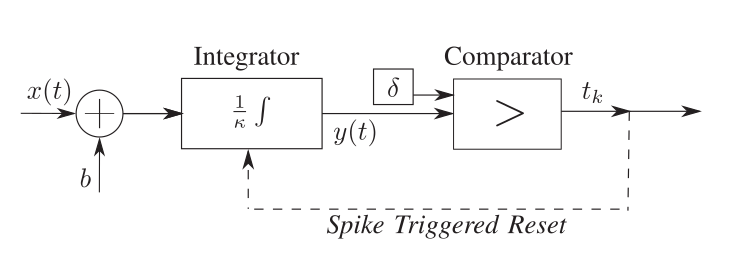
\includegraphics[width = 14cm , height = 6cm]{1.jpg}
    \caption{TEM}
    \label{fig:my_label}
\end{figure}

\textbf{NOTE:} The TEM can be defined in a slightly different way , wherein the integrator is initialized to $\delta$ and if the integrator output is less than $-\delta$ the time is recorded. Even in this case the analysis will proceed along the same lines to that in this paper.
\subsection{Stability of a TEM}
For all input signals $x(t)$, $t\in\mathbb{R}$ with $\vert x(t) \vert \leq c < b$ the TEM is stable,i.e., $\vert y(t) \vert \leq \delta$ $\forall t $, $t\in\mathbb{R}$. 
This fact is apparent from the way the TEM functions , clearly the output of the integrator $y(t)$ is bounded between $-\delta$ and $\delta$.
\subsection{Iterative reconstruction of band-limited Signals}
\begin{theorem}\label{th21}
A signal $x(t)$ can be perfectly reconstructed from samples obtained from a TEM if it satisfies following conditions:
\begin{itemize}
    \item $x(t)$ has to be square integrable\footnote{a function is said to be square integrable on $\mathbb{R}$ if $\int_{-\infty}^{\infty}{\vert x(t) \vert}^2dt < \infty$.This function is said to be in $L^2(\mathbb{R})$.}.
    \item It must be bounded,i.e., $\vert x(t)\vert < c$ and $b < c$.
    \item $x(t)$ must be band-limited(maximum frequency: $\omega$) and $w < \frac{\pi(b-c)}{2k\delta}$.
\end{itemize}
\end{theorem}
\vspace{0.2cm}
\begin{flushleft}
The following equation is straightforward from the way a TEM functions:   
\end{flushleft}
\begin{equation}
     \int_{t_k}^{t_{k+1}}x(u)du = 2k\delta - b(t_{k+1}-t_{k})
\end{equation}
\subsubsection{Upper and Lower bounds on trigger times}
We know that,
\begin{center}
    $|x(t)| \leq c$\\
    $-c \leq x(t) \leq c$\\
    $\displaystyle-c\int_{t_k}^{t_{k+1}}dt \leq \int_{t_k}^{t_{k+1}}x(t)dt \leq c\int_{t_k}^{t_{k+1}}dt$\\
\end{center}    
Using $(1)$
\begin{center}
    $-c(t_{k+1}-t_k) \leq 2k\delta - b(t_{k+1}-t_k) \leq c(t_{k+1}-t_k)$
    \\
    $(b-c)(t_{k+1}-t_k) \leq 2k\delta \leq (b+c)(t_{k+1}-t_k)$
\end{center}
$\Rightarrow$
\begin{center}
    $(t_{k+1} - t_k) \leq \frac{2k\delta}{b-c}$\\
    \& $(t_{k+1}-t_k) \geq \frac{2k\delta}{b+c}$
\end{center}
Therefore, we have
\begin{equation}
    \frac{2k\delta}{b+c} \leq t_{k+1} - t_k \leq \frac{2k\delta}{b-c}
\end{equation}
As we can see the difference between two successive trigger times is bounded , this fact will be useful in the following section.
\vspace{0.2cm}\\
\textbf{***}It is recommended to go through \textbf{APPENDIX A} before moving on to the next section.

\subsubsection{Algorithm for iterative reconstruction}
Consider the following reconstruction operator:\\
\begin{equation}
    R(y(t)) = \sum_{k\in\mathbb{Z}}[g(t-s_k)\int_{t_k}^{t_{k+1}}y(u)du]
\end{equation}
where $s_k = \frac{(t_k+t_{k+1})}{2}$ and $g(t) = \frac{sin(\omega t)}{\pi t}$.
\vspace{0.2cm}\\
\begin{flushleft}
Consider the operator $R^*$ on bandlimited signals given by,
\end{flushleft}

\begin{equation}
    R^*x = \sum_{k\in\mathbb{Z}}x(s_k)f_k(t)
\end{equation}
where $f_k(t) = (g*1_{[t_k,t_{k+1}]})(t)$ represents a Low pass filter with impulse response $g$ , with input as a rectangular pulse.\\
\begin{lemma}
$R$ and $R^*$ are adjoint operators.
\end{lemma}
\begin{proof}
$R$ and $R^*$ are said to be adjoint if ,
\begin{equation*}
    \langle Rx,y \rangle = \langle x,R^*y \rangle
\end{equation*}
with the inner product given by convolution operation.
Also if $x$ is bandlimited by $\omega$ then the filter will let it pass through,i.e.,\\
\begin{equation*}
    g*x = x 
\end{equation*}
Now using the above equation, properties of convolution ooperation( distributive, associative, commutative) we can prove the lemma. 
\[
    \langle Rx,y \rangle = \langle \sum_{k\in\mathbb{Z}}\int_{t_k}^{t_{k+1}}x(t)dt g(t-s_k),y \rangle
\]
\[
    = \sum_{k\in\mathbb{Z}}\int_{t_k}^{t_{k+1}}x(t)dt y(s_k)
\]
\[
    = \langle x , \sum_{k \in \mathbb{Z}}1_{[t_k,t_{k+1}]}y(s_k) \rangle
\]
As we know 
\[  
    = \langle g*x,\sum_{k\in\mathbb{Z}}1_{[t_k,t_{k+1}]}y(s_k)\rangle
\]
\[
    = \langle x,\sum_{k\in\mathbb{Z}}g*1_{[t_k,t_{k+1}]}y(s_k)\rangle
\]
\[  
    = \langle x,R^*y \rangle
\]
Thus, $R$ and $R^*$ are adjoint.
\end{proof}
\begin{flushleft}
\textbf{NOTE:} Inequalities given in \textbf{APPENDIX B} have been used in the proof of following lemma
\end{flushleft}
\begin{lemma}
\begin{equation}
    \|I - R\| \leq r
\end{equation}
where $I$ is the identitiy operator and $r = \frac{2k\delta\omega_0}{(b-c)\pi}$
\end{lemma}
\begin{proof}
Consider the operator $LPF$ given in \textbf{APPENDIX A}, we can write $R^*$ as:
\begin{equation*}
    R*(x) = \sum_{k\in\mathbb{Z}}x(s_k)LPF1_{[t_k,t_{k+1}]}  
\end{equation*}
as $x*g = x$ or $LPFx = x$:
\[
    \norm{x-R^*x}^2 = \norm{LPFx - \sum_{k\in\mathbb{Z}}x(s_k)LPF1_{[t_k,t_{k+1}]}}
\]
\[
    \leq \norm{\sum_{k\in\mathbb{Z}}[x-x(s_k)]1_{[t_k,t_{k+1}]}}^2
\]
\[
    \norm{x-R^*x}^2 \leq \sum_{k\in\mathbb{Z}}\int_{t_k}^{t_{k+1}}\abs{x(t)-x(s_k)}^2dt
\]
in order to apply Wirtinger's inequality we split the integral into two parts so that the value of integrand is zero at one of the integral limits,i.e.,
\[
    \int_{t_k}^{t_{k+1}}\abs{x(t)-x(s_k)}^2dt = \int_{t_k}^{s_{k}}\abs{x(t)-x(s_k)}^2dt + \int_{s_k}^{t_{k+1}}\abs{x(t)-x(s_k)}^2dt
\]
clearly $\abs{x(t)-x(s_k)}^2 = 0$ when $t = s_k$, thus both the integrands on $LHS$ satisfy the condition required to apply Wirtinger's Inequality.\\
Applying Wirtinger's Inequality we get,
\[
    \int_{t_k}^{t_{k+1}}\abs{x(t)-x(s_k)}^2dt \leq \frac{4}{\pi^2}(s_k - t_k)^2\int_{t_k}^{s_k}\abs[\Big]{\frac{dx(t)}{dt}}^2dt + \frac{4}{\pi^2}(t_{k+1} - s_k)^2\int_{s_k}^{t_{k+1}}\abs[\Big]{\frac{dx(t)}{dt}}^2dt
\]
We know that $s_k = \frac{t_k+t_{k+1}}{2}$ , so ,
\begin{equation*}
    s_k - t_k = t_{k+1} - s_k = \frac{t_{k+1} - t_k}{2}
\end{equation*}
from (2) in \textbf{1.3.1} we know,
\begin{equation*}
    t_{k+1} - t_k \leq \frac{2k\delta}{b-c}
\end{equation*}
$\Rightarrow$
\[
      \int_{t_k}^{t_{k+1}}\abs{x(t)-x(s_k)}^2dt \leq \frac{4k^2{\delta}^2}{\pi^2(b-c)^2}\int_{t_k}^{t_{k+1}}\abs[\Big]{\frac{dx(t)}{dt}}^2dt  
\]
\[
    \norm{x-R^*x}^2 \leq \frac{4k^2{\delta}^2}{\pi^2(b-c)^2}\norm{\frac{dx(t)}{dt}}^2
\]
Now using Bernstein's Inequality , 
\[
    \norm{\frac{dx(t)}{dt}}^2 \leq \omega_0^2\norm{x(t)}^2
\]
thus, we have
\[
    \norm{x-R^*x} \leq r\norm{x}
\]
where $r = \frac{2k\delta\omega_0}{\pi(b-c)} $\\
Since $\norm{R} = \norm{R^*}$ \footnote{refer {https://proofwiki.org/wiki/Norm\_of\_Adjoint}}
\[
    \norm{x-Rx} \leq r\norm{x}
\]
\[
    \norm{I-R} \leq r
\]
\end{proof}
\begin{theorem}\label{th22}
Now the signal $x(t)$ can be reconstructed by:
\begin{enumerate}
    \item Initialize $x_0$ as $R(x)$,i.e., 
    \begin{equation}
        x_0=R(x)
    \end{equation}
    \item Find $x1,x2,....$ by doing the following
    \begin{equation}
        x_{l+1} = x_l + R(x-x_l)
    \end{equation}
    \item This series $x1,x2,.....$ will converge to $x(t)$ if it satisfies the conditions given in \textbf{Theorem \ref{th21}}.
\end{enumerate}
\end{theorem}

\begin{proof}
The following can be proved by induction
\begin{equation}
    x_l = \sum_{k=0}^l(I-R)^kRx
\end{equation}
from \textbf{lemma 1.2} $\norm{I-R}\leq r$, if the signal $x(t)$ satisfies the conditions given in \textbf{Theorem \ref{th21}} then , $r < 1$.
$\Rightarrow$
\[
    \lim_{l \to \infty}x_l = \sum_{k\in\mathbb{N}}(I-R)^kRx = R^{-1}Rx = x
\]
Thus the series clearly converges to $x(t)$
\end{proof}

\subsection{Matrix formulation}
Let $G,H,q$ denote the following matrices:
\begin{equation*}
    G = [g(t-s_k)]_{k\in\mathbb{Z}} 
\end{equation*}
\begin{equation*}
    H = [H_{lk}]_{l,k\in\mathbb{Z}} = [\int_{t_l}^{t_{l+1}}g(t-s_k)dt]_{l,k\in\mathbb{Z}} \\ 
\end{equation*}
\begin{equation*}   
    q = [\int_{t_k}^{t_{k+1}}x(t)dt]_{k\in\mathbb{Z}}
\end{equation*}
A corollary of the \textbf{Theorem \ref{th22}} is as follows:\\
\begin{corollary}
the bandlimited signal $x(t)$ can be perfectly recovered from its associated trigger times $(t_k)$,$k\in\mathbb{Z}$,as\\
\begin{equation}
    x(t) = \lim_{l\to\infty}x_l(t) = G^TH^+q
\end{equation}
where $G^T$ denotes the transpose of $G$ and $H^+$ denotes the pseudo inverse\footnote{} of $H$.
and ,\\
\begin{equation*}
    x_l(t) = G^TP_lq
\end{equation*}
where $P_l$ is given by:\\
\begin{equation*}
    P_l = \sum_{k=0}^l(I-G)^k
\end{equation*}
where $I$ denotes the identity matrix.
\end{corollary}

\section{POCS Algorithm}
\subsection{Convex Set}
\begin{defn}
In a vector space, a set $C$ is called convex set iff $\forall\overrightarrow{x}$,$\overrightarrow{y} \in C$ ,\\
$\Rightarrow$\begin{center}
    $\lambda\overrightarrow{x} + (1-\lambda)\overrightarrow{y} \in C$ \\
    $0\leq\lambda\leq1$
\end{center}
\end{defn}
\begin{theorem}
The intersection of two convex sets is a convex set .
\end{theorem}
\begin{proof}
Consider two convex sets $C_1,C_2$ and their intersection $C_1\cap C_2$ , let $\overrightarrow{x},\overrightarrow{y}$ be arbitrary vectors in $C_1\cap C_2$,
\[
    \overrightarrow{x},\overrightarrow{y} \in C_1\cap C_2
\]
$\Rightarrow$
\[
    \overrightarrow{x},\overrightarrow{y} \in C_1
\]
\[
    \overrightarrow{x},\overrightarrow{y} \in C_2
\]
As $C_1$ and $C_2$ are convex sets,
\[
    \lambda\overrightarrow{x} + (1-\lambda)\overrightarrow{y} \in C_1
\]
\[
    \lambda\overrightarrow{x} + (1-\lambda)\overrightarrow{y} \in C_2
\]
\[
    0\leq\lambda\leq1
\]
$\Rightarrow$
\[
    \lambda\overrightarrow{x} + (1-\lambda)\overrightarrow{y} \in C_1\cap C_2
\]
Thus, by definition $C_1\cap C_2$ is a convex set.
\end{proof}
\subsection{Projection Onto a Convex Set}
\begin{theorem}
For every (closed) convex set $C$ and every vector $\overrightarrow{x}$ in a Hilbert space\footnote{refer Appendix A}, there is a unique vector in $C$, closest to $x$.
This vector denoted by $P_cx$, is called the projection of $\overrightarrow{x}$ onto $C$.\footnote{This is a famous result of convex analysis also known as \textbf{Hilbert Projection Theorem}.}
\end{theorem}
\begin{proof}

\end{proof}

\subsection{The Algorithm}
Consider $N$ convex sets $C_1,C_2,...,C_N$ which are subsets of a Hilbert space $X$ and let the projection operators onto this set be given by $P_1,P_2,...,P_N$.\\
\begin{flushleft}
The algorithm functions to solve the following problem:\\
find a solution for $x$, called $\hat{x} \in C_1\cap C_2\cap.....\cap C_N$ i.e., find a solution for $x$ that lies in the intersection of the $N$ convex sets.\\
The POCS algorithm does this by selecting an arbitrary initial value and then by alternatingly projecting it onto the sets $C_1,C_2,....,C_N$ using the projection operators $P_1,P_2,.....,P_2$. This is known to converge to some $\hat{x} \in C_1\cap C_2\cap.....\cap C_N$.Thus, the approach is also known as \textbf{Alternating POCS}.
\end{flushleft}
\begin{itemize}
    \item Start with an arbitrary value $x_0$.
    \item Generate the following sequence
    \begin{equation}
        x_{i+1} = P_{C_1}(P_{C_2}(.....P_{C_N}(x_i)))
    \end{equation}
\end{itemize}
\subsubsection{Some properties of the POCS algorithm}
\begin{lemma}
Alternating POCS among $N$ convex sets with a non-empty intersection will converge to a point common to all sets.
\end{lemma}
\begin{lemma}
Alternating POCS among 2 non-intersecting convex sets will converge to the point in each set closest to the other,i.e., the solution will keep oscillating between these two points. This is known as the \textbf{limit cycle}.
\end{lemma}
\begin{lemma}
Alternating POCS among 3 or more convex sets with an empty intersection will converge to a \textbf{limit cycle}.\\
\end{lemma}
\begin{flushleft}
\textbf{NOTE:}
\end{flushleft}
Different order of projection operations will produce different limit cycles. If we start by projecting onto set-$1$ and then project onto set-$2$ this wont be same as projecting first onto set-$2$ and then onto set-$1$. Both the cases will result in different limit cycles.
\subsubsection{Simultaneous weighted projection}
There is a slightly different version of POCS.In some cases even though the sets do not have any intersection we might require that the algorithm still converges but as we have seen if the sets do not intersect it goes into a limit cycle. In order to avoid this we use the following algorithm instead of Alternating-POCS:
\begin{itemize}
    \item Take projections of the vector $x_0$ onto each set.
    \item Take the average(or weighted average) of all the projections.
    \item Repeat the above steps till it converges.
\end{itemize}
This allows us to obtain a minimum mean square error solution in cases where the sets do not intersect.\\
Often we may have to make a trade off between different constraints,i.e.,we may not be able to find a solution which satisfies all the requirements(constraints). In that case we will have to choose which constraint is more important(priority).If we look at the convex sets as representing different constraints, then rather than taking average we can take a weighted average where the weights represent the priority of different constraints. The basic operation in this approach is as follows:
\begin{equation}
    P_s\overrightarrow{x} = \sum_{n=1}^{N}w_nP_n\overrightarrow{x}
\end{equation}
where
\begin{center}
    $w_n$ : weight or priority
\end{center}
\section{Reconstruction using POCS}
In order to be able to apply the POCS algorithm we need to know the convex sets and their respective projection operators.\\ 
Consider the operator $R$ defined in \textbf{section 2.3.2} (3) , the operator can also be defined as follows:
\begin{equation}
    R(y(t)) = \Big[\sum_{k\in\mathbb{Z}}\delta(t-s_k)\int_{t_k}^{t_{k+1}}y(u)du\Big]*g(t)
\end{equation}
now consider another operator $B$ defined as follows:
\begin{equation}
    B(y(t)) = \sum_{k\in\mathbb{Z}}\delta(t-s_k)\int_{t_k}^{t_{k+1}}y(u)du
\end{equation}
The operator $B$ takes an input signal and maps it to the set of signals which have same integral as the input between $t_k$ and $t_{k+1} \forall k \in \mathbb{Z}$.
\begin{defn}
Consider the set of all signals $y(t)\in L^2(\mathbb{R})$ that satisfy $\int_{t_k}^{t_{k+1}}y(u)du = \int_{t_k}^{t_{k+1}}x(u)du, \forall k \in \mathbb{Z}$, let this set be $C_{1}$.
\end{defn}
All the signals within the set $C_1$ generate the same set of \textbf{spike-times($t_k$)} when passed through a \textbf{TEM}.\\
As we already know $g(t) = \frac{sin(\omega_0 t)}{\pi t}$ , this is the impulse response of an ideal low pass filter(\textbf{LPF}) with cutoff frequency $\omega_0$. So if we convolve a signal with $g(t)$ it will be mapped to the set of bandlimited signals with maximum frequency $w$.\\
\begin{defn}
Let the set of all bandlimited signals with maximum frequency $\omega_0$ be denoted by $C_{\omega_0}$.
\end{defn}
The operator $R$ now takes an input signal and maps it first onto the set $C_1$ and then onto the set $C_{\omega_0}$\\
So recursively applying $R$ is same as alternately projecting onto two convex sets, the set of bandlimited signals and the set of functions which give the spike times ${t_k,k\in\mathbb{Z}}$.However the range of operator $B$ does not lie in a Hilbert space, thus we cannot directly apply POCS\footnote{given in the paper , assumed this to be true.}.In order to solve this, it has been assumed that input signals are in $L^2(\mathbb{R})$ and consider the operator $B_1$:
\begin{equation}
    B_1(y(t)) = \sum_{k\in\mathbb{Z}}\int_{t_k}^{t_{k+1}}y(u)du \frac{1}{t_{k+1}-t_k}\mathds{1}_{[t_k,t_{k+1})}(t)
\end{equation}
where $\mathds{1}_{[t_k,t_{k+1})}(t)$ is one when $t\in[t_k,t_{k+1})$ and zero otherwise. The only difference between $B_1$ and $B$ is that $B_1$ produces signals that are in $L^2(\mathbb{R})$, which is a Hilbert space.\\
We clearly see that we can solve this problem using POCS provided that the sets $C_1$ and $C_{\omega}$ are convex and we know the projection operators onto these sets and that these operators are firmly nonexpansive\footnote{}.

\begin{lemma}
$C_{\omega_0}$ is a convex set
\end{lemma}
\begin{proof}
Consider any two arbitrary signals(or vectors) $x,y \in C_{\omega_0}$, 
\begin{equation*}
    x_1,x_2 \in C_{\omega_0}
\end{equation*}
Let , $0 \leq \lambda \leq 1$
consider the signal $x_3 = \lambda x_1 + (1-\lambda) x_2 $ , the fourier transform of $z$ is given by:
\begin{equation*}
    X_3(\omega) = \lambda X_1(\omega) + (1-\lambda) X_2(\omega)
\end{equation*}
if $|\omega|$ $>$ $\omega_0$ then by defenition of $C_{\omega_0}$ ,
\begin{equation*}
    X_1(\omega) = 0 
\end{equation*}
\begin{equation*}
    X_2(\omega) = 0
\end{equation*}
Thus, 
\begin{equation*}
    X_3(\omega) = 0 , \forall |\omega| > \omega_0
\end{equation*}
i.e., $x_3 \in C_{\omega}$
Thus , $C_{\omega}$ is a convex set.
\end{proof}

consider the projection operator $P_{\omega_0}$ onto the set $C_{\omega_0}$ given by:
\begin{equation}
    P_{\omega}(y(t)) = y(t)*g(t) 
\end{equation}

\begin{lemma}
$P_{\omega}$ is a firmly nonexpansive projection operator onto $C_{\omega}$.
\end{lemma}

\begin{lemma}
$C_1$ is a convex set
\end{lemma}
\begin{proof}
Consider any two arbitrary signals(or vectors) $x_1,x_2 \in C_{1}$, 
\begin{equation*}
    x_1,x_2 \in C_{1}
\end{equation*}
$\Rightarrow$
\[
    \int_{t_k}^{t_{k+1}}x_1(t)dt = \int_{t_k}^{t_{k+1}}x_2(t)dt = \int_{t_k}^{t_{k+1}}x(t)dt
\]
Let , $0 \leq \lambda \leq 1$
consider the signal $x_3 = \lambda x_1 + (1-\lambda) x_2 $
now,
\[
    \int_{t_k}^{t_{k+1}}x_3(t)dt = \lambda\int_{t_k}^{t_{k+1}}x_1(t)dt + (1-\lambda)\int_{t_k}^{t_{k+1}}x_2(t)dt
\]
\[
    = \lambda\int_{t_k}^{t_{k+1}}x(t)dt + (1-\lambda)\int_{t_k}^{t_{k+1}}x(t)dt 
\]
\[
    = \int_{t_k}^{t_{k+1}}x(t)dt
\]
Thus by definition of $C_1$, $x_3 \in C_1$\\
Therefore, $C_1$ is a convex set.
\end{proof}

consider the projection operator $P_1$ onto the set $C_1$ given by:
\begin{equation}
    P_{1}(y(t)) = y(t) + B_1(x(t)-y(t))
\end{equation}

\begin{lemma}
$P_1$ is a firmly nonexpansive projection operator onto $C_1$.
\end{lemma}


Now we can reconstruct the signal by using the POCS algorithm as follows:
\begin{itemize}
    \item initialize $x_0$ as:
    \begin{equation}
        x_0 = B_1(x(t))*g(t) 
    \end{equation}
    \item Generate the series:
    \begin{equation}
        x_{l+1} = P_{\omega}(P_{1}(x_l))
    \end{equation}
\end{itemize}
As we have already seen this will converge to $x(t)$.

\section{M-Channel TEM}
\textbf{$M$} denotes the number of TEMs.\\
An $M$-channel TEM consists of $M$ TEMs , with the same parameters $k,\delta,b$ but each with a different integrator shifts. The difference between outputs of two integrators(integrator shifts) is given by $\alpha_1,\alpha_2,........,\alpha_M$.Where $\alpha_i$ are given by:
\begin{equation}
    y_{i+1}(t) = ( y_i(t) + \alpha_i ) mod 2\delta, i = 1,.....,M-1
\end{equation}
\begin{equation}
    y_{1}(t) = ( y_M(t) + \alpha_M ) mod 2\delta ,
\end{equation}
where $y_i(t)$ denotes the output of integrator in $i^{th}$ TEM at time $t$.\\
One important property of an M-channel TEM is $(\sum_i\alpha_i)mod2\delta = 0$.This arises from the way $\alpha_i$'s are defined. If we expand the above equations recursively we obtain $y_1(t) = y_1(t) + \sum_i\alpha_imod2\delta$ and from this the property follows.\\
If we assume that all the shifts are non-zero then the following is also clear:
\begin{equation}
    t_{k-1}^{(i+1)} < t_k^{(i)} < t_k^{(i+1)} \forall k,\forall i = 1,......,M-1 
\end{equation}
\begin{equation}
    t_k^{(1)} < t_k^{(M)} < t_{k+1}^{(1)} \forall k
\end{equation}
where $t_k^{(i)}$ denotes the spike times given by $i^{th}$ TEM.
The equations (20) and (21) state that all the TEMs spike in a given order,i.e., first the TEM$1$ spikes followed by TEM$2$ and so on , once all the $M$-TEMs spike then the same repeats again.

\subsection{M-channel Reconstruction of band-limited signals using POCS}
The advantage of using an M-channel TEM instead of single channel is that bandwidth of input signals can be increased.\\
The input signal can be successfully reconstructed if,
\begin{equation}
    \omega_0 < \frac{\pi(b-c)}{2k\alpha_{max}}
\end{equation}
where $\alpha_{max} = max(\alpha_1,.....,\alpha_M)$, The bandwidth will be maximum when $\alpha_{max}$ is minimum. If all the integrators were spaced in such a way that $\alpha_{max} = \alpha_i , \forall i = 1....M$ , then the bandwidth is M-times that of single channel.\\
However this is the case even if the spacings are not same unless the are non-zero,i.e.,
\begin{equation}
    \omega < \frac{M\pi(b-c)}{2k\delta}
\end{equation}
Consider the sets $C_i , i = 1,...... ,M$ where $C_i$ denotes the set of all signals that give the same spike-times when passed through the $i^{th}$TEM.Thus all $C_i$'s are convex.The projection operator onto these sets is defined the same way as in \textbf{Lemma 3.4}.
The reconstructed signal must belong to all these sets , and to the set of all bandlimited signals with maximum frequency $\omega_0$ , and all these sets are convex, now we can use the POCS algorithm to reconstruct the signal.\\
We will use the weighted projection version of the POCS algorithm. As the reconstructed signal must belong to all $C_i$s the weights will all be equal , so we'll simply take the average of all projection operators and define a new operator as follows:
\begin{equation*}
    P_{1....M} = \frac{1}{M}\sum_{i=1}^{M}P_i 
\end{equation*}
Now we have to project this onto the set $C_{\omega}$ to complete reconstruction.i.e.,
\begin{equation*}
    R_{1...M}(x) = P_{\omega}(P_{1....M}(x))
\end{equation*}
where $R_{1...M}$ is the reconstruction operator.
Using the definitions given in previous sections
\begin{equation*}
    R_{1...M}(x) = P_{\omega}\Big(\frac{1}{M}\sum_{i=1}^{M}B_{i}(x(t))\Big)
\end{equation*}
where $B_i$ is the following operator
\begin{equation}
    B_i(y(t)) = \sum_{k\in\mathbb{Z}}\int_{t_k^(i)}^{t_{k+1}^(i)}y(u)du\frac{1}{t_{k+1}-t_k}\mathds{1}_{[t_k,t_{k+1})}(t).
\end{equation}
Now $R_{1...M}$ can be given as
\begin{equation*}
    R_{1...M}(x) = \frac{1}{M}\sum_{i}^{M}B_i(x(t))*g(t)
\end{equation*}
Consider the operators
\begin{equation*}
    R_i = B_i(x(t))*g(t) , \forall i = 1,....,M
\end{equation*}
These are same as the reconstruction operator for single channel TEM using POCS.Simply $R_{1...M}$ given by their average.
\begin{equation}
    R_{1...M}(x) = \frac{1}{M}\sum_{i}^{M}R_i
\end{equation}
Now the signal can be reconstructed as follows:
\begin{itemize}
    \item initialize $x_0$ as $x_0 = R_{1...M}(x)$
    \item then generate the following series
    \begin{equation}
        x_{l+1} = x_l + R_{1...M}(x-x_l)
    \end{equation}
\end{itemize}
This series will converge to $x(t)$.
\section{Matrix formulation}
Let $t_k^{~}$ denote the vector containing spike times of all TEMs.\\
Let $GM,HM,qM$ denote the following matrices:
\begin{equation}
    GM = [\mathds{1}_{[t_k^{~},t_{k+M}^{~}]}(t)*g(t)]_{k\in\mathbb{Z}}
\end{equation}
\begin{equation}
    HM = [HM_{lk}]_{l,k\in\mathbb{Z}} = \Big[\int_{t_k^{~}}^{t_{k+M}^{~}}\mathds{1}_{[t_k^{~},t_{k+M}^{~}]}(t)*g(t)\Big]_{l,k\in\mathbb{Z}}
\end{equation}
\begin{equation}
    qM = \Big[\int_{t_k^{~}}^{t_{k+M}^{~}}x(t)dt\Big]_{k\in\mathbb{Z}}
\end{equation}
then similar to the case of reconstruction in a single channel TEM,
\begin{equation}
    x(t) = \lim_{l\to\infty} x_l(t) = GM^THM^+qM
\end{equation}
where,
\begin{equation}
    x_l(t) = GM^T\Big(\sum_{k=0}^l(I-HM)^k\Big)qM
\end{equation}

\appendix
\section*{\begin{center}
    APPENDIX A\\Hilbert Spaces and Low pass filter as a projection operator
\end{center}}
\begin{defn}
A non-negative real-valued function $\|.\|$ defined on a vector space $V$ is called a norm if $\forall x,y \in V$ \\
\begin{equation}
    \|x\| = 0 \Leftrightarrow x = 0
\end{equation}
\begin{equation}
    \|x+y\| \leq \|x\| + \|y\|
\end{equation}
\begin{equation}
    \|\alpha x\| = |\alpha|\|x\|
\end{equation}
\end{defn}

\begin{defn}
If every Cauchy sequence in the space converges then the normed linear space is called complete.
\end{defn}

\begin{defn}
An inner product on a vector space $V$ over $\mathbb{C}$, is a complex-valued function $\langle .,. \rangle$ defined on $V\times V$ to $\mathbb{C}$ such that
\begin{equation}
    \langle x+y,z \rangle = \langle x,z \rangle + \langle y,z \rangle    
\end{equation}
\begin{equation}
        \langle \alpha x,y \rangle = \alpha \langle x,y \rangle
\end{equation}
\begin{equation}
    \langle x,y \rangle = \langle y,x \rangle^{*}
\end{equation}
\begin{equation}
    \langle x,x \rangle \geq 0,\langle x,x \rangle = 0
\end{equation}
\end{defn}

\begin{defn}
A complete vector space whose norm is induced by an inner product is called a Hilbert Space\footnote{A Hilbert space generalizes the idea of a Euclidean space(2Dimensional and 3dimensional) to higher dimensional spaces. roughly it can be looked at as generalizing the idea of distance.}.
\end{defn}

\begin{defn}
Operator $B$ and $B^{*}$ defined on a Hilbert space $\mathcal{H} \rightarrow \mathcal{H}$ are said to be adjoint if $\forall x,y \in \mathcal{H} ,$\\
\begin{equation}
    \langle Bx,y \rangle = \langle x,B^{*}y \rangle
\end{equation}
\end{defn}



\begin{defn}
Let $L^{2}(\mathbb{R})$ be the Hilbert space of bounded energy functions and let $B$ be the sybset of bandlimited signals(functions). The projection operator $LPF$ maps an arbitary function in $x \in L^2$ into a bandlimited function in $B$ as ,
\begin{equation}
    LPFx = (g*x)(t) ;
\end{equation}
where $g(t) = \frac{sin(wt)}{\pi t}$ .\\
\end{defn}
Simply, if we notice $g(t)$ is the impulse response of a low pass filter with cut-off frequency $w$ ,i.e., the projection operator $LPF$ is a low pass filter .


\newpage
\section*{\begin{center}
    APPENDIX B\\Bernstein's inequality\\ Wirtinger's inequality
\end{center}}
\begin{lemma}
if a signal $x(t)$ is defined on $\mathbb{R}$ and is bandlimited with maximum frequency $\omega_0$ then $\frac{dx(t)}{dt}$ is also bandlimited and,
\begin{equation}
    \norm{\frac{dx(t)}{dt}} \leq \omega_0\|x(t)\|
\end{equation}
This is known as \textbf{Bernstein's inequality}.
\end{lemma}
\begin{proof}
    We know that the fourier transform of $\frac{dx(t)}{dt}$ is given by:
    \begin{equation}
        \mathcal{F}\Big(\frac{dx(t)}{dt}\Big) = j\omega X(\omega) 
    \end{equation}
    where $X(\omega)$ denotes fourier transform of $x(t)$.\\
    $x(t)$ is bandlimited\\
    $\Rightarrow$ 
    \begin{equation}
        X(\omega) = 0 , \forall \omega > \omega_0
    \end{equation}
    $\Rightarrow$
    \begin{equation}
        \mathcal{F}\Big(\frac{dx(t)}{dt}\Big) = 0 , \forall \omega > \omega_0
    \end{equation}    
    Thus, $\frac{dx(t)}{dt}$ is also bandlimited.\\
    Now , using Parseval's theorem:
    \begin{center}
        $\norm{\frac{dx(t)}{dt}}^2 = \frac{1}{2\pi} \norm{{F}\Big(\frac{dx(t)}{dt}\Big)}^2 = \frac{1}{2\pi}\norm{j\omega X(\omega)}^2$\\
    \end{center}
    We know that $X(\omega)$ is non-zero only when $\omega \in [-\omega_0 , \omega_0 ]$ 
    Thus considering only this range of $\omega$ , we get the following inequality:
    \begin{equation*}
        \norm{\omega} \leq \omega_0
    \end{equation*}
    Using the above inequality , fact that $\norm{j} = 1$ and properties of norm we get:
    \begin{center}
        $\norm{\frac{dx(t)}{dt}}^2 \leq \frac{\omega_0^2}{2\pi}\norm{X(w)}^2$
    \end{center}
    Now using parsevals inequality we obtain:
    \begin{center}
        $\norm{\frac{dx(t)}{dt}}^2 \leq \omega_0 \norm{x(t)}^2$
    \end{center}
    From this Bernstein's inequality follows.
\end{proof}

\begin{lemma}
    If $x(t),\frac{dx(t)}{dt} \in L^2(a,b)$\footnote{a signal $x(t)$ is said to be in $L^2(a,b)$ if it is square integrable in the interval $[a,b]$,i.e.,  $x(t) \in L^2(a,b)$ iff $\int_a^b|x(t)|^2dt < \infty$.} and either $f(a) = 0$ or $f(b) = 0$, then
    \begin{equation}
        \int_a^b|x(t)|^2dt \leq \frac{4}{\pi^2}(b-a)^2\int_a^b\abs[\Big]{\frac{dx(t)}{dt}^2}dt
    \end{equation}
    This is known as \textbf{Wirtinger's Inequality}
\end{lemma}

\section*{\begin{center}
    REFERENCES
\end{center}}
[1] https://robertmarks.org/Presentations/POCS/index.htm\\
\end{document}